\documentclass[12pt,oneside]{book}
\usepackage[vcentering,dvips]{geometry}
\geometry{papersize={210mm,297mm},total={165mm,230mm}}
\special{pdf: pagesize width 165mm height 230mm}
\usepackage{graphicx}
\usepackage{graphics}
\usepackage{fancyhdr}
\usepackage{epsfig}
\usepackage{subfigure}
\usepackage{tabularx}
\usepackage{amssymb}
\usepackage{graphicx}
\graphicspath{{images/}}
\usepackage{graphics}
\usepackage{fancyhdr}
\usepackage{epsfig}
\usepackage{subfigure}
\usepackage{tabularx}

\usepackage{titleref}
\usepackage{multirow} 
\usepackage{url}
\usepackage{picture}
\usepackage{verbatim}
\usepackage{xfrac}
\usepackage{physics}
\usepackage{makecell}
\usepackage[running, displaymath, mathlines]{lineno}
% \linenumbers
% \linenumbers


\usepackage[font={footnotesize}, bf]{caption}
\usepackage[pdf]{pstricks}
\usepackage{hyperref}

\hypersetup{
  colorlinks   = true, %Colours links instead of ugly boxes
  urlcolor     = blue, %Colour for external hyperlinks
  linkcolor    = blue, %Colour of internal links
  citecolor   = red %Colour of citations
}
\usepackage{appendix}
\usepackage[utf8]{inputenc}
\usepackage[T1]{fontenc}
% \usepackage[czech]{babel}
% \languageattribute{czech}{split}

\usepackage{tikz}
    \usetikzlibrary{patterns}
    \usepackage{pgfplots}

\usepackage{nicefrac}
    
\usepackage{cmap}
\usepackage{natbib}
\bibliographystyle{model2-names}
% \biboptions{authoryear}

\usepackage{xcolor}
\definecolor{siva}{RGB}{100,200,255}
\usepackage[framemethod=TikZ]{mdframed}
\mdfdefinestyle{nevyz}{%
    linecolor=blue,
    outerlinewidth=1pt,
    roundcorner=10pt,
    innertopmargin=\baselineskip,
    innerbottommargin=\baselineskip,
    innerrightmargin=10pt,
    innerleftmargin=10pt,
%     backgroundcolor=gray!30!white}
    backgroundcolor=siva}

   \mdfdefinestyle{vyz}{%
    linecolor=red,
    outerlinewidth=4pt,
    roundcorner=10pt,
    innertopmargin=\baselineskip,
    innerbottommargin=\baselineskip,
    innerrightmargin=10pt,
    innerleftmargin=10pt,
    backgroundcolor=white}
%     backgroundcolor=white} 
    
\renewcommand{\baselinestretch}{1.5}

\newcommand{\HRule}{\rule{\linewidth}{0.5mm}}
\newcommand{\SRule}{\rule{\linewidth}{0.2mm}}
%\newcommand{\dd}{\textrm{d}}
\newcommand{\nd}{2$^{\textrm{nd}}$~}
\newcommand{\st}{1$^{\textrm{st}}$~}
\newcommand{\xth}{$^{\textrm{th}}$~}

\newcommand{\cdr}{convection-diffusion-reaction equation}

\newcommand{\highlight}[1]{%
  \colorbox{red!50}{$\displaystyle#1$}}
  
\newcommand{\highlightr}[1]{%
  \colorbox{red!60}{$\displaystyle#1$}}
  
  
\newcommand{\highlightb}[1]{%
  \colorbox{blue!40}{$\displaystyle#1$}}

\newcommand{\highlightg}[1]{%
  \colorbox{green!70}{$\displaystyle#1$}}
  
\newcommand{\highlightc}[1]{%
  \colorbox{cyan!40}{$\displaystyle#1$}}
  \newcommand{\fs}{\footnotesize}

    \newcommand{\dg}{$^{\circ}$}
    
\newcommand\restr[2]{{% we make the whole thing an ordinary symbol
  \left.\kern-\nulldelimiterspace % automatically resize the bar with \right
  #1 % the function
  \vphantom{\big|} % pretend it's a little taller at normal size
  \right|_{#2} % this is the delimiter
  }}

\def\listofsymbols{\input{symbols} \clearpage}
\def\addsymbol #1: #2#3{$#1$ \> \parbox{4.323in}{#2 \dotfill \pageref{#3}}\\}
\def\newnot#1{\label{#1}} 
\def\tvdots{\raisebox{3pt}{$\scalebox{.75}{\vdots}$}}
%\begin{document}
\pagestyle{fancy}

\setcounter{secnumdepth}{3} 
\setcounter{tocdepth}{3} 

\rhead{\scriptsize\textsf{\rightmark}}
\chead{}

\lfoot{}
\cfoot{}
\rfoot{}

% Macro for 'List of Symbols', 'List of Notations' etc...
\def\listofsymbols{\input{symbols} \clearpage}
\def\addsymbol #1: #2#3{$#1$ \> \parbox{4.323in}{#2 \dotfill \pageref{#3}}\\}
\def\newnot#1{\label{#1}} 
\def\tvdots{\raisebox{3pt}{$\scalebox{.75}{\vdots}$}}
\usepackage{footnote}
\usepackage[bottom]{footmisc}
\usepackage{amsmath}
\usepackage{mathrsfs}

\usepackage{tikz}
\newcommand*\circled[1]{\tikz[baseline=(char.base)]{
            \node[shape=circle,draw,inner sep=2pt] (char) {#1};}}
            
\usepackage[scientific-notation=true]{siunitx} %VVV
\sisetup{round-mode = places, round-precision = 3} %VVV

 \usepackage[framemethod=TikZ]{mdframed}
\mdfdefinestyle{important}{%
    linecolor=blue,
    outerlinewidth=1pt,
    roundcorner=10pt,
    innertopmargin=\baselineskip,
    innerbottommargin=\baselineskip,
    innerrightmargin=10pt,
    innerleftmargin=10pt,
%     backgroundcolor=gray!30!white}
    backgroundcolor=siva}

   \mdfdefinestyle{pedantic}{%
    linecolor=red,
    outerlinewidth=4pt,
    roundcorner=10pt,
    innertopmargin=\baselineskip,
    innerbottommargin=\baselineskip,
    innerrightmargin=10pt,
    innerleftmargin=10pt,
    backgroundcolor=white}
%     backgroundcolor=white} 

\newenvironment{columns}[1][]
        {\setkeys{columns@col}{#1}
         \noindent\begin{minipage}{\textwidth}}
        {\end{minipage}\vspace{.5cm}}

\newenvironment{column}[1]
        {\begin{minipage}[t]{#1}}
        {\end{minipage}}

\usepackage{multirow}
    
    
    \usepackage{lmodern}
    \usepackage{courier}
    
\usepackage{listings}
\lstset{language=[90]Fortran,
basicstyle=\linespread{0.85}\footnotesize\ttfamily,
  keywordstyle=\bfseries,
  commentstyle=\color{olive}\textit,
  numbers=left,
    stepnumber=1,
    showstringspaces=false,
    tabsize=1,
    breaklines=true,
    breakatwhitespace=false,
  morekeywords=[1]{class, abstract},
  keywordstyle=[1]{\bfseries\color{blue}}
%   basicstyle=\ttfamily,
%   keywordstyle=\bfseries,
%   commentstyle=\color{green},
%   morecomment=[l]{!\ }, 
%   numbers=left,
%     stepnumber=1,
%     showstringspaces=false,
%     tabsize=1,
%     breaklines=true,
%     breakatwhitespace=false
}

\begin{document}





\begin{titlepage}

 
\begin{center}
 
 

 
{\textsf{\bfseries{Faculty Environmnetal Sciences, Czech University in Prague, \\ Faculty of Civil Engineering, Czech Technical University in Prague}}}\\[5.5cm]



\textsf{\LARGE Advanced Computational Mathematics}\\[1.0cm]
 

\textsf{ \large Juliana  Arbelaez Gaviria \\ Johanna Ruth Bl\"ocher \\ Gustavo Enrique Castillero Cardenas, \\ Batuhan Der \\ 
Mijael Rodrigo  Vargas Godoy \\ Eva Meli\v{s}ov\'a \\ Michal Kur\'a\v{z} \\ Petr Mayer} 
 
 \vspace{50mm}
{
 \large
\bf \sf 2020 }
\end{center}
\end{titlepage}



\chapter{1st class -- problem definition}

\section{Our equation}

Many problems in engineering practice can be described by 
\begin{equation}
\label{oureq}
 - (p u')' + q u = f,
\end{equation}
 where $u$ is the solution, $p$ and $q$ are coefficients, $f$ is a scalar function.  It is known that solution of \eqref{oureq} 1) exist and 2) is unique, if $p > 0$ for the given boundary conditions
 \begin{equation}
 \label{dirbc}
  \begin{split}
   u(0) &= u_{0}, \\
    u(1) & = u_{1},
  \end{split} 
 \end{equation}
or 
\begin{equation}
\label{dirneubc}
 \begin{split}
      u(0) &= u_{0}, \\
    u'(1) & = \vec{q}_{1},
 \end{split} 
\end{equation}
or 
\begin{equation}
\label{robinbc}
 \begin{split}
  \alpha_{0}u(0) + \alpha_{1}u'(0) &= a ,\\
     \beta_{0}u(1) + \beta_{1}u'(1) &= b ,
 \end{split} 
\end{equation}
where \eqref{dirbc} is a combination of Dirichlet conditions, \eqref{dirneubc} is a combination of Dirichlet and Neumann conditions, and \eqref{robinbc} is a combination of mixed (Robin) conditions.

For more spatial dimensions \eqref{oureq} is formulated as
\begin{equation}
\label{oureqD}
- \nabla \cdot (\mathbf{P} \nabla u)  + qu = f .
\end{equation}

\section{Approximate solution}
Since exact solution is often unknown, as direct integration is in 
many real world cases  impossible, an approximate solution to \eqref{oureq} or \eqref{oureqD} can be constructed out of polynomials and so
\begin{equation}
\label{bencheq}
 u \approx p_{n}(x) = \sum_{i=0}^{n}\pi_{i} x^{i} 
\end{equation}


if $n = 1$ then coefficients $\pi_{0,1}$ can be simply obtained from boundary conditions and so
\begin{equation}
 \begin{split}
  u_{0} &= p_{1}(0) = \pi_{0}, \\
   u_{1} &= p_{1}(1) = \pi_{1},
 \end{split} 
\end{equation}
it is apparent, that definition of $\pi_{0,1}$ satisfying the given Dirichlet conditions has no relation to our equation!

Let us assume the following benchmark example
\begin{equation}
\label{benchsin}
 -u'' + 4u  = \sin 3x.
 \end{equation}
It is known that the exact solution is  
\begin{equation}
u(x) = \alpha \exp(2x) + \beta \exp(-2x)+ \frac{1}{13} \sin 3x,  
\end{equation}
where $\alpha$ and $\beta$ are defined by boundary conditions setup. If 
we set $\alpha = 0$ and $\beta = 1$, then the boundary conditions state 
that
\begin{equation}
\begin{split}
  u(0) &= 1, \\
  u(1) &= \exp(-2) + \frac{\sin 3}{13}
\end{split}
\end{equation}

With increasing value of $n$ we can define a well known method for approximating differential equations -- {\it collocation method}.

The method can be demonstrated as follows.

For polynomial approximation of degree $n=1$, solution is 
approximated by \begin{equation}p_{1}(x) = \pi_{1}x + \pi_{0}\end{equation}, and so $\pi_{0}=1$. 
The coefficient $\pi_{1}$ is obtained from the second boundary 
condition and so
\begin{equation}
\begin{split}
 p(1)_{1} = \pi_{1}\times 1.0 + \pi_{0} = \exp(-2) + \frac{\sin 3}{13} 
 \Rightarrow \pi_{1} = \exp(-2) + \frac{\sin 3}{13}  - 1.
 \end{split}
\end{equation}
It is apparent that definition of $\pi_{0,1}$ had no relation to 
\eqref{benchsin}. And so we shoudl search for higher degree 
approximation.

If $n=2$, then 
\begin{equation}p_{2}(x) = \pi_{2}x^{2} +\pi_{1}x + \pi_{0}\end{equation},
then let's select some interior point for which the equation 
\eqref{benchsin} is 
satisfied, eg. $x_{int}=0.5$.

Then we can constitute the following system of linear equations for 
$\pi_{0,1,2}$.

\begin{equation}
 \label{systemcolloc} 
 \begin{split}
  \pi_{0} &= 1 \qquad \mbox{ \fs (1st boundary condition)} \\
  \pi_{0} + \pi_{1} \times 1.0 + \pi_{2} \times 1.0^{2} &=  \exp(-2) + 
  \frac{\sin 3}{13} \qquad  \mbox{ \fs (2nd boundary condition)} \\
  \pi_{0} + \pi_{1}\times 0.5 + \pi_{2} \times 0.5^{2} &= \sin (3 
  \times 0.5) \qquad \mbox{ \fs (interior point)}.
 \end{split} 
\end{equation}
Analogicaly for $n=3$, approximation polynomial is then
\begin{equation}p_{3}(x) = \pi_{3}x^{3} + \pi_{2}x^{2} +\pi_{1}x + 
\pi_{0},\end{equation} interior points will be then
$x_{int_{1}}=\sfrac{1}{3}$ , and $x_{int_{2}}=\sfrac{2}{3}$. Similar 
system to \eqref{systemcolloc} is then assembled. Convergence of the 
collocation method for the selected benchmark problem is apparent from 
figure~\ref{collocconv}.
\begin{figure}
\centering
 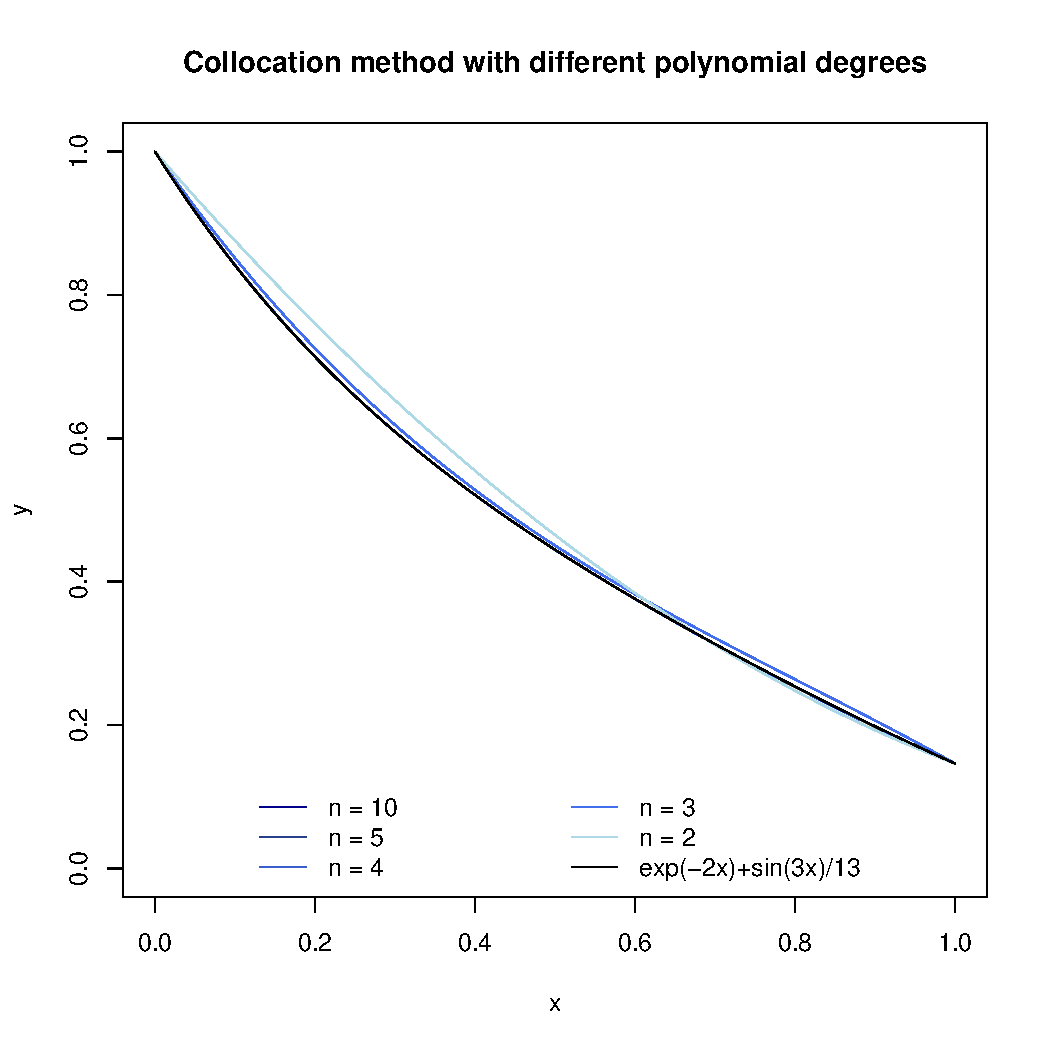
\includegraphics[width=9cm]{images1/collocation_adv_numerics.pdf}
 \label{collocconv}
 \caption{Approximating benchmark problem \eqref{benchsin} with 
 polynomials constructed with collocation method.}
\end{figure}

The collocation method is an analogy to Lagrangian interpolation with the same quality properties  -- possibly divergent prone!!. A disputable approach, error is measured at discrete points, but we are searching for a continuous approximation!.


Another approach for defining the error continuously is {\it least square method} (later it will be defined as {\it least-square-finite-element-method} (here after LSFEM).

In order to simplify our notations our problem \eqref{oureq} will be expressed in terms on differential operator
\begin{equation}
%\label{oureq}
 \overbrace{- (p u')' + q u = f}^{Lu}.
\end{equation}
let $u_{h}$ be the approximation of $u$. The LSFEM method measures approximation error as
\begin{equation}
 \varepsilon = \int\limits_{\Omega} (L u_{h} - f )^{2} \dd \Omega,
\end{equation}
and so the solution is obtained by setting
\begin{equation}
  \int\limits_{\Omega} (L u_{h} - f )^{2} \dd \Omega \leadsto \mbox{min}.
\end{equation}

And so \eqref{bencheq} if $\alpha=0$ and $\beta=1$ can be solved as 
\begin{equation}
 \int\limits_{0}^{1} (  -u'' + 4u  - \sin 3x )^{2} \dd x \leadsto \mbox{min} \wedge p(0) = 1 \, \& \, p(1) = \exp(-2) + \sin\left(\frac{3}{13}\right),
\end{equation}
which is just a constraint minimization.

Another approach is 
\begin{equation}
 \int\limits_{0}^{1} (  -u'' + 4u  - \sin 3x )^{2} \dd x  + P_{0} (p_{n}(0)-u_{0})^{2} + P_{1} (p_{n}(1) - u_{1})^{2}\leadsto \mbox{min} ,
 \end{equation}
where $P_{0,1}$ are penalization constants, by setting $P_{0,1}$ values we define how important satisfying the boundary conditions is, theoretically if $P_{0,1} \leadsto \infty$ the boundary conditions are exactly satisfied, however, our solution became independent on the governing equation.

The bottle neck of these methods is that it is difficult to relate these residuals to physical properties. And so yet another approach will be defined here. Let's define scalar product and our operator $L$ as
\begin{equation}
\begin{split}
 (L(u),v) &= (v, L(u)) \\
  L(u + v) &= L(u) + L(v) \\
  L(\alpha u) &= \alpha L(u) \\
  (L(u),v) &\ge c(u,v), \; \exists c>0.
\end{split}
\end{equation}
The last condition implies that our operator is {\it positive definite}.

Then let us define 
\begin{equation}
 E(u) = (L(u),v) - 2(f,v),
 \end{equation}
 where $E$ is energy functional -- an energy of our system. There is a proof, which says that minimizing $E$ leads to a best approximation of our solution. Such method is referred to as Ritz method. 
 
 Problem with using just polynomials starts with more dimensions. It is still relatively simple to find polynomial satisfying given boundary conditions for rectangular.
 
 \begin{center}
 \begin{tikzpicture}
\draw [draw=black] (3.0,3.0) rectangle (0.3,0.3);
%\filldraw [fill=Peach, draw=black] (11.1,5) rectangle (0.3,0.3);
%\filldraw [fill=RedOrange, draw=black] (11.1,4.5) rectangle (0.3,0.3);
\end{tikzpicture}
\end{center}
 
 
 \begin{equation}
  -\Delta u = 1 , \; \Omega = (0,1) \times (0,1), \; \restr{u}{\Gamma} = 0, 
 \end{equation}
 which is 
 \begin{equation}
  u_{h} = x(1-x)(1-y) \sum_{i}^{n} \sum_{i}^{n}\pi_{i,j}x^{i}y^{i}. 
 \end{equation}
 
 
 But issues start with L-shape $\Omega = (0,1) \times (0,1) - (\sfrac{1}{2},1) \times (\sfrac{1}{2},1) $

 
 \begin{center}
 \rotatebox{0}{
 
\includegraphics[width=4cm]{images1/lshape.eps}}
 \end{center}

 It is impossible to find polynomial, which satisfies the given boundary conditions.
 

 

\chapter{2st class }

Let's define the following differential equation 

\begin{equation}
	Lu = f
\end{equation}

where the linear operator $Lu$ is defined as 
\begin{equation}
	Lu = -u''
\end{equation}

 and using the Laplacian or Laplace operator
 
\begin{equation}
Lu = - \laplacian{u} = - \Delta u
\end{equation}

A boundary-value problem can be defines then as

\begin{equation}
\label{example1}
\begin{split}
- \Delta u & = 1 \\
u & = 0  \quad  x \in \partial{\Omega}
\end{split}
\end{equation}

where  the domain is define 
\begin{equation}
\Omega = (0,1) \times (0,1) - (\sfrac{1}{2},1) \times (\sfrac{1}{2},1) 
\end{equation}

graphically, 

 \begin{center}
	\rotatebox{0}{
		
\includegraphics[width=4cm]{images2/discretization.eps}}
\end{center} 

and the task is to approximate \eqref{example1} by polynomials $\in C^2$ or differentiable up to second derivative. This is a minimization problem, where it can be used LSM 

\begin{equation}
S(u) = \int_{\Omega} (Lu - f)^2 \rightarrow min
\end{equation}

or RITZ method based on minimize the energy of the system as follows

\begin{equation}
E(u) = \int_{\Omega} Lu\cdot u - 2fu  \rightarrow min
\end{equation}

Defining a space $V$ where  $V_n \subset V$ and $V_n = \zeta_{exp}(\varphi_1, \varphi_2, ..., \varphi_n)$ where $\varphi_n$ is a polynomial of degree n, and $dim(V_n) < n$, and the approximate solution of the differential equation is 

\begin{equation}
u_n = \sum_{i=1}^{n} \alpha_i \varphi_i
\end{equation}

The energy of the system is defined as

\begin{equation}
E(u_n) = \int_{\Omega}\left(  L \sum_{i=1}^{n} \alpha_i \varphi_i\right)  \sum_{j=1}^{n} \alpha_j\varphi_j - 2f  \sum_{i=1}^{n} \alpha_i \varphi_i 
\end{equation}

\begin{equation}
E(u_n) = \int_{\Omega}  \sum_{i=1}^{n} \sum_{j=1}^{n}  \alpha_i  \alpha_j L  \varphi_i \varphi_j - 2 \sum_{i=1}^{n} \alpha_i f \varphi_i 
\end{equation}

\begin{equation}
E(u_n) =  \sum_{i=1}^{n} \sum_{j=1}^{n}  \alpha_i  \alpha_j \int_{\Omega}   L \varphi_i \varphi_j - 2 \sum_{i=1}^{n} \alpha_i \int_{\Omega}  f \varphi_i 
\end{equation}

In matrix form

\begin{equation}
E(u_n) = \alpha^T \mathbf{A} \alpha - 2 \alpha^T b
\end{equation}

where 

\begin{equation}
A_{ij} = \int_{\Omega}   L \varphi_i \varphi_j 
\end{equation}
 
 and 
 
 \begin{equation}
 b_{i} = \int_{\Omega}  f \varphi_i
 \end{equation}


We will defined $u_{n1}, u_{n2}, ..., u_{nn}$ but the question is $$\lim_{i\to\infty }u_{ni}$$ exist or not, since there can be smooth functions where the limit is not part of the same space $V$. 

The space $V$ is defined as  $\norm{\cdot}$: $V \rightarrow  \real_0^+$ with the following properties

\begin{enumerate}
	\item  $\norm{u} \geq 0$
	\item  $\norm{u} = 0  \quad u=0$
	\item  $ \norm{\alpha u} = \alpha \norm{u}$
\end{enumerate}

Def: \\
$\lim u_{n} = u$ $\leftrightarrow \forall \varepsilon > 0 \quad  \exists n_0 \quad \forall n >n_0 : \quad \norm{u-u_n} < \varepsilon$

 \begin{center}
	\rotatebox{0}{
		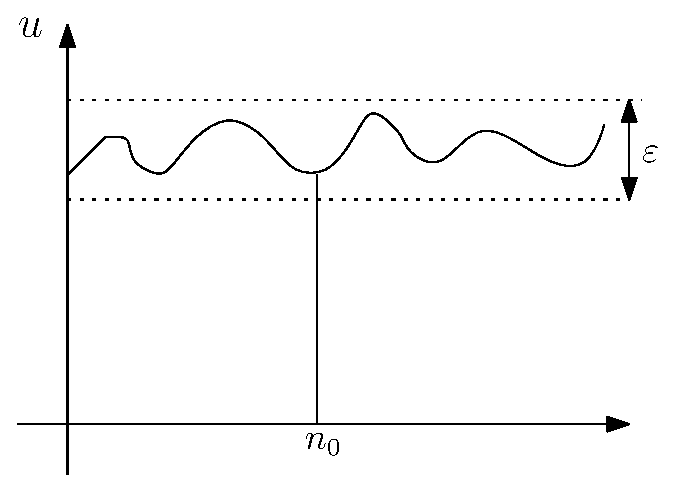
\includegraphics[width=4cm]{images2/derivative.eps}}
\end{center} 

The more common norms are $\norm{\cdot}_p$ and $\norm{\cdot}_\infty$, defined as follows for $V= C_{<0,1>}$
\begin{equation}
	\begin{split}
		\norm{u}_\infty & =   \max_{x\in(0,1)}\abs{u(x)} \\
		\norm{u}_p & = \left( \int_{0}^{1} \abs{u(x)}^p\right)^{\frac{1}{p}}
	\end{split}
\end{equation}

Def: \\
$u_n$ is cauchy $\leftrightarrow \forall \varepsilon > 0 \quad  \exists n_0 \quad \forall n,m >n_0 : \quad \norm{u_n-u_m} < \varepsilon$

any convergent sequence is cauchy but not every cauchy sequence is convergent. 

If we defined $\bar{V} = \bar{\bar{V}}$ is a closed space of $V$ where we add all the cauchy sequences, named $H_1$. $H_1$ is a space that can contain continuous but not smooth function. In other words, there are functions that do not have second derivative.  Notice then, for  $v \in H_1$ , $Lv = f $ is not satisfy. 

The Galerkin method states 
\begin{equation}
	\forall v \quad (Lu,v) = (f,v)
\end{equation}

Assuming homogeneous Dirichlet condition $u(0)=u(1)=0$, we have

\begin{equation}
\int_{0}^{1} (-(pu')' + qu)\cdot v = \int_{0}^{1} f\cdot v
\end{equation}

Proceeding with  integration by parts

\begin{equation}
\int_{0}^{1} -(pu')v' + quv  = \int_{0}^{1} f\cdot v
\end{equation}

\begin{equation}
\int_{0}^{1} (-(pu')' v +\int_{0}^{1} qu v =   - pu'v \Big|_0^1  +   \int_{0}^{1} pu'v' + \int_{0}^{1} fv
\end{equation}
	
\begin{equation}
  \int_{0}^{1} pu'v' + qu v  =  \int_{0}^{1} fv
\end{equation}

which is equivalent to the weak form 

\begin{equation}
(u,v)_L = (f,v)
\end{equation}

The weak solution is not related to the original problem, moreover, notice it is no longer required continuity in the second derivative since $u''$  is not par of the solution. 



\end{document}
